\chapwithtoc{Introduction}
	\ac{TPC} is a~type of gaseous detector that detects charged particle trajectories by measuring the~position and drift time of ions created in the~gas (details are given in section~\ref{sec:tpc}). The~energy of such particles can be determined thanks to the~curvature of their trajectory in the~magnetic field.
	
	The~goal of this thesis is to develop an~algorithm for the~reconstruction of charged particle trajectory and energy in an~atypic \ac{TPC} (with orthogonal electric and magnetic fields, i.e. \ac{OFTPC}) used in the~X17 project in \ac{IEAPCTU}. Furthermore, we present the~results of testing this algorithm with different samples of simulated data. In the~future, we also wish to test this algorithm by measuring real particles with known energy distribution. In order to achieve this, we use the~Garfield++ toolkit~\cite{Garfield++} in combination with the~ROOT~framework~\cite{ROOT}. We run some of our more demanding simulations on MetaCentrum.
	
	The~X17 project in \ac{IEAPCTU} aims to reproduce measurements of anomalous behavior in the distribution of angular correlation of pairs produced by the~\ac{IPF} mechanism during the~decay of certain excited nuclei (\iso{Be}{8},~\iso{C}{12}~and~\iso{He}{4}) observed by the~ATOMKI group in Hungary. 
	
	\textcolor{red}{Add citations MetaCentrum, X17 project, VdG, ATOMKI papers. Maybe also TPC, IPF, ...}
	
	\section{ATOMKI Measurements}
	\textcolor{red}{Short summary of results of measurements in ATOMKI.}
	
	\section{X17 IEAP CTU}
	\label{sec:IEAP}
	\textcolor{red}{Short description of our detector. Why we use atypic TPC. Magnetic field simulations in Maxwell. Description of the coordinate system used in this thesis (+ figure).}
	
	\begin{figure}
		\centering
		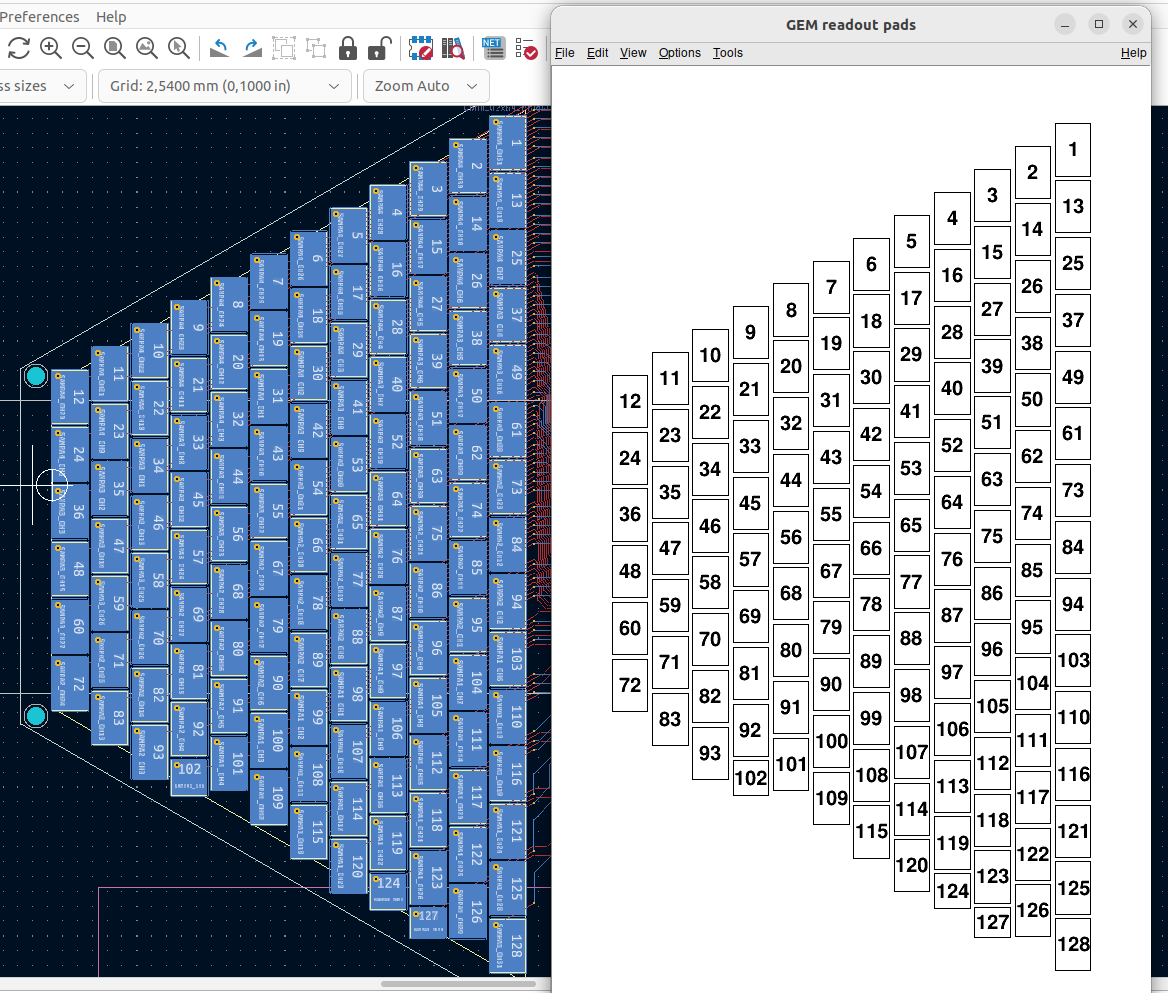
\includegraphics[width=0.8\textwidth]{padlayout.png}
		\caption{Pad layout of the TPC. \textcolor{red}{Swap for better image.}}
		\label{fig:padlayout}
	\end{figure}